\section{Model}
\label{sec:model}

The classical fair queuing problem is that given input bandwidths $IB_i$ with
weights $W_i$ for all clients calculate allocated bandwidths $AB_i$ for each
client such that:  

{\bf 1. Congestion Freedom:}  The sum of the allocated bandwidths does not
exceed the bandwidth $B$ of the outbound link. This is rarely specified
explicitly as a classical hardware scheduler only operates after each packet is
transmitted, so the model ensures there is no congestion.

{\bf 2. Strong Fair Allocation: } Divide $B$ among active clients in proportion
to their weights $W_i$.

\begin{figure}[t]
\center
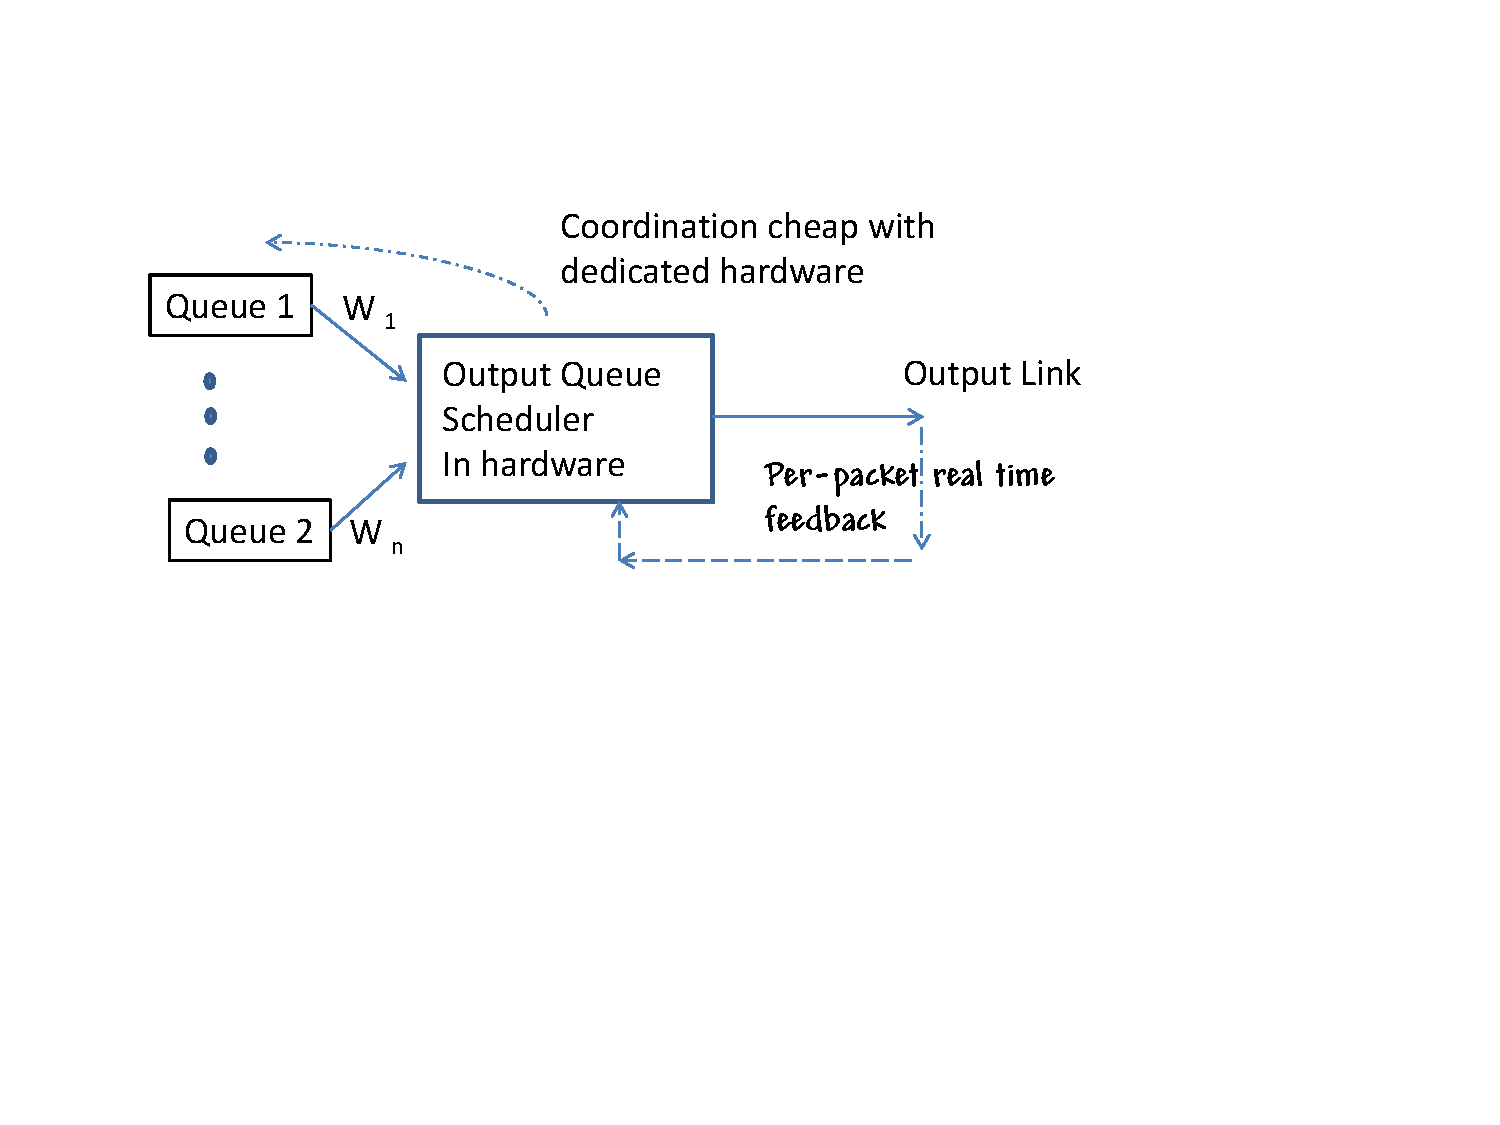
\includegraphics[width=\columnwidth,trim=6mm 90mm 20mm 10mm]{figures/standardqosmodel}
\caption{Standard Fair queuing model}
\label{fig:qosmodel}
\vspace{-2mm}
\end{figure}

There are many algorithms for this classical fair queuing model including
Deficit Round Robin, Start-time Fair Queuing, and Worst Case Weighted Fair
Queuing~\cite{drr, stfq,w2fq, qfq}. These algorithms make two implicit
assumptions. First, they assume that after transmission of a packet the link
alerts the hardware scheduler that then chooses the next packet to transmit. The
second assumption is that the scheduler is able to keep up with link speed.
Both these assumptions are reasonable in the scenarios where fair queuing is
traditionally investigated - i.e. routers and switches.

However, in our scenario the model is the one shown in
Figure~\ref{fig:vmqosmodel}.  The first thing that has changed when going from
Figure~\ref{fig:vmqosmodel} to Figure~\ref{fig:qosmodel} is that the feedback
loop between the link and the scheduler has now become a batched feedback loop.
Modern NICs use mechanisms like Large Send Offload (LSO) to minimize overhead.
Thus they can only generate one send-complete notification for a group of
packets, instead of generating one for every individual packet.  Without a
per-packet feedback loop, a DRR-like implementation in software will receive
transmit completion notifications in bursts.  Not only will these bursts cause
transmit jitter, but the bursts can also be very far in between, with respect to
the rate of packet arrival, causing the queues to overflow and packets to be
dropped. Second, even if the NIC could invoke the scheduler on a per-packet
basis, the cost of running the scheduler after every packet departure will be
prohibitive. It typically takes at least one full core to saturate a 40Gbps link,
if not more. 
 
\begin{figure}
\centering
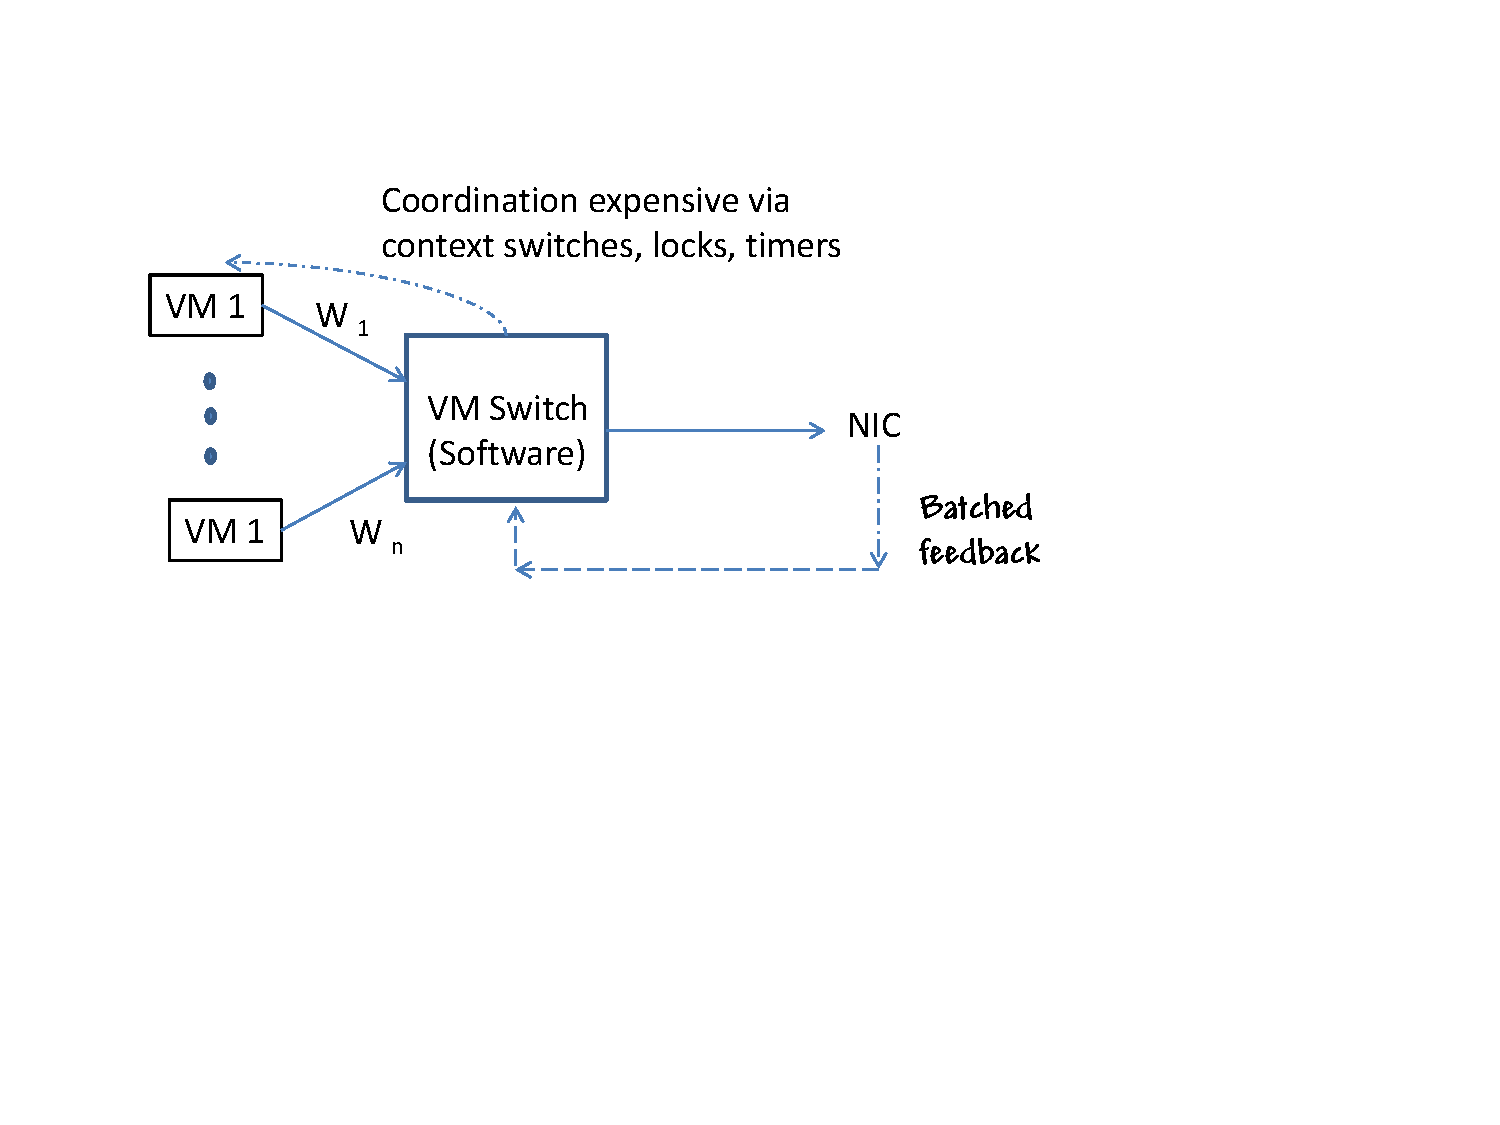
\includegraphics[width=\columnwidth, trim=6mm 90mm 20mm 10mm]{figures/vmqosmodel}
\caption{Model for VM Fair Queuing}
\label{fig:vmqosmodel}
\vspace{-3mm}
\end{figure}

We also need to deal with some additional constraints in our scenario.
The software entity that schedules packets out of the queues need to
ensure that packets are en-queued to the NIC's transmit buffer in the same order
that they are de-queued from the different queues.  

There are two options to achieve this. First, the software could use a handle to
the NIC's transmit buffer.  This requires strong coordination between the
software module and the NIC's driver.  For a software implementation on top of a
hardware abstraction layer in a general-purpose OS that needs to work across a
large variety of NIC vendors (e.g. the NDIS abstraction layer in Windows), this
is not currently a feasible option.  

A second alternative is that the software entity has to be single-threaded so
that each packet are processed sequentially through the entire software stack
from when it is de-queued from the software queues until it is queued to the
NIC's transmit buffer. This requires a single processor to handle all packet
processing through the entire software stack. This is not a scalable solution at
multi-gigabit speed.  Additionally, having to process packets on a single thread
forces packets that were processed on different processors to be then processed
on a different single processor, leading to cache misses, which can lead to
added latency.

A way out of these difficulties is to divide the scheduler into two enties as
shown in Figure~\ref{fig:macroscheduler}.   The macroscheduler runs only every
$T$ seconds and hence can run on a single thread.   The microschedulers, by
contrast, run on every packet based on tokens allocated by the microscheduler.   

\begin{figure}
\centering
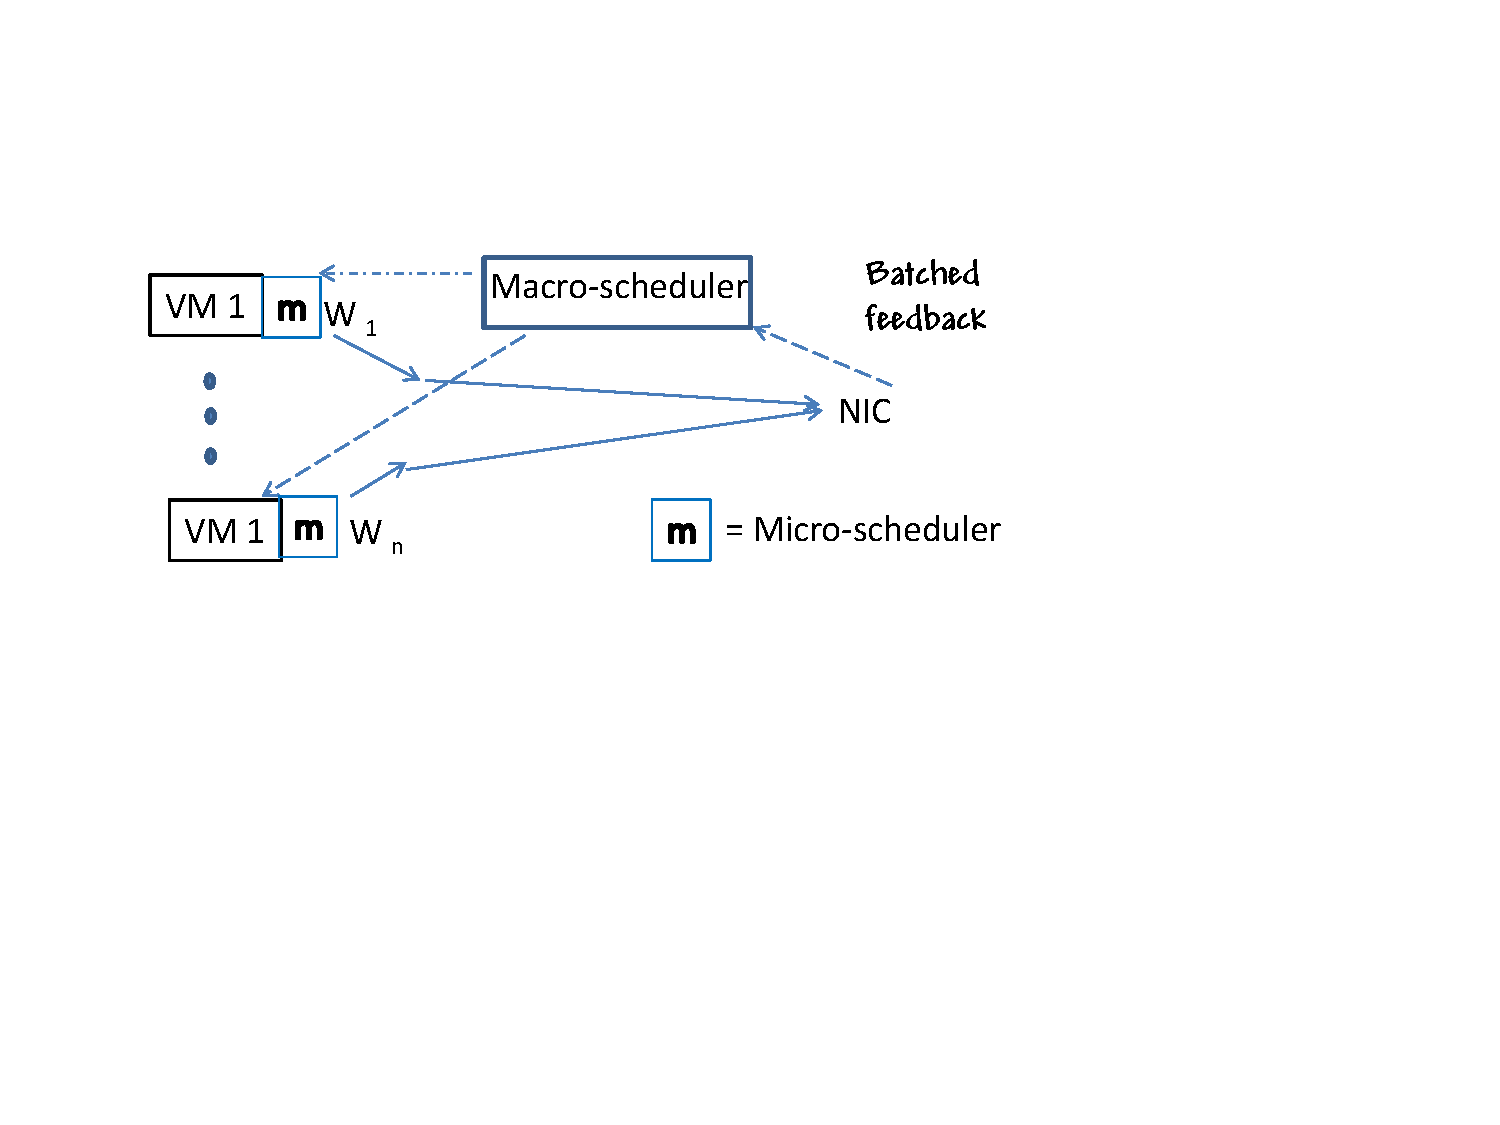
\includegraphics[width=\columnwidth, trim=6mm 90mm 20mm 10mm]{figures/macroschedule}
\caption{Macroscheduler/Microscheduler model}
\label{fig:macroscheduler}
\vspace{-3mm}
\end{figure}

While this model reduces overhead it has obvious drawbacks because allocations
can only occur in units of $T$ seconds.   Thus we have two measures $T_{inc}$
which defines the worst case time for a VM to increase to its guaranteed
bandwidth, and $T_{dec}$ which is the worst case time after a VM decreses below
its allocation till the unused bandwidth is distributed to all active VMs. 
